%============================================================
% Template LaTeX Proyek Akhir Sarjana Terapan
% Politeknik Elektronika Negeri Surabaya (PENS)
% Berdasarkan Panduan Buku PA SarjanaTerapan A4 Rev05
%============================================================

\documentclass[12pt, a4paper, twoside, openright, fleqn]{report}

%------------------------------------------------------------
% PACKAGES
%------------------------------------------------------------
\usepackage[T1]{fontenc}
\usepackage[utf8]{inputenc}
\usepackage{mathptmx}          % Times New Roman (teks + math)
\usepackage{setspace}          % Spasi 1.5
\usepackage{geometry}          % Margin
\usepackage{graphicx}          % Gambar
\usepackage{caption}           % Caption gambar/tabel
\usepackage{float}             % Posisi float [H]
\usepackage{tabularx}          % Tabel fleksibel
\usepackage{booktabs}          % Tabel profesional
\usepackage{array}             % Kolom tabel custom
\usepackage{amsmath}           % Persamaan matematika
\usepackage{amssymb}
\usepackage{xcolor}            % Warna
\usepackage{colortbl}          % Warna sel tabel (rowcolor)
\usepackage{tikz}              % Gambar vektor (materai, dll)
\usepackage{fancyhdr}          % Header/footer kustom
\usepackage{emptypage}         % Halaman kosong tanpa header/footer
\usepackage{tocloft}           % Kustomisasi daftar isi
\usepackage{titlesec}          % Format judul bab/subbab
\usepackage{indentfirst}       % Indentasi paragraf pertama
\usepackage{parskip}           % Jarak antar paragraf
\usepackage{cite}              % Sitasi IEEE
\usepackage{url}               % URL pada daftar pustaka
\usepackage{hyperref}          % Hyperlink (matikan warna)
\usepackage{ragged2e}
\usepackage{microtype}
\usepackage{enumitem}          % List kustom
\usepackage{pdfpages}          % Include halaman pengesahan eksternal
\usepackage{etoolbox}
\usepackage{tabularray}

% --- PENGATURAN PERSAMAAN MATEMATIKA ---
\setlength{\mathindent}{10mm}

\setlength{\abovedisplayskip}{-15pt}
\setlength{\belowdisplayskip}{0pt}
\setlength{\abovedisplayshortskip}{0pt}
\setlength{\belowdisplayshortskip}{0pt}

\makeatletter
\renewcommand{\tagform@}[1]{\maketag@@@{\bfseries\itshape(#1)\@@italiccorr}}
\makeatother

%------------------------------------------------------------
% WARNA
%------------------------------------------------------------
\definecolor{pensbiru}{RGB}{0, 47, 167}    % #002FA7
\definecolor{penskuning}{RGB}{255, 193, 7} % Garis emas cover

%------------------------------------------------------------
% GEOMETRI HALAMAN (mirror margin)
%------------------------------------------------------------
\geometry{
  a4paper,
  top    = 3cm,
  bottom = 3cm,
  inner  = 4cm,   % kiri untuk halaman ganjil (binding)
  outer  = 3cm,   % kanan untuk halaman ganjil
  twoside
}

%------------------------------------------------------------
% SPASI
%------------------------------------------------------------
\onehalfspacing   % 1,5 spasi sesuai panduan

%------------------------------------------------------------
% INDENTASI & PARAGRAF
%------------------------------------------------------------
\setlength{\parindent}{1.27cm}
\setlength{\parskip}{0pt}

%------------------------------------------------------------
% FORMAT JUDUL BAB & SUB-BAB
%------------------------------------------------------------
% 1. Format Judul Bab:
\titleformat{\chapter}[display]
{\centering\fontsize{14}{17}\bfseries}
{BAB \thechapter}
{0pt}
{}
\titlespacing*{\chapter}{0pt}{0pt}{18pt}

% 2. Format Subbab (Section):
\titleformat{\section}
{\fontsize{14}{17}\bfseries}
{\thesection}
{1em}
{}
\titlespacing*{\section}{0pt}{16pt}{0pt}

% 3. Format Sub-subbab (Subsection):
\titleformat{\subsection}
{\fontsize{12}{14}\bfseries}
{\thesubsection}
{1em}
{}
\titlespacing*{\subsection}{0pt}{12pt}{4pt}

%------------------------------------------------------------
% CAPTION GAMBAR & TABEL (ukuran 11pt, tebal, rata tengah)
%------------------------------------------------------------
\captionsetup[figure]{
  labelfont  = {it},
  textfont   = {it},
  font       = {small},   % 11pt ≈ small dalam dokumen 12pt
  justification = centering,
  skip       = 6pt,
  name       = Gambar,
  labelsep   = space
}
\captionsetup[table]{
  labelfont  = {it},
  textfont   = {it},
  font       = {small},
  justification = centering,
  skip       = 6pt,
  position   = above,
  name       = Tabel,
  labelsep   = space
}

\renewcommand{\tablename}{Tabel}

% Pengaturan global format Tabularray (Berlaku untuk tblr dan longtblr)
\SetTblrInner{
  hlines, vlines,                                  % Garis kotak otomatis
  row{1} = {bg=gray!20, font=\bfseries, halign=c}, % Header otomatis: Abu-abu, Bold, Center
  rowhead = 1,                                     % Ulangi header jika tabel terpotong halaman
}

% Penomoran gambar/tabel per-bab (Gambar 3.1, Tabel 4.2, dst.)
\renewcommand{\thefigure}{\thechapter.\arabic{figure}}
\renewcommand{\thetable}{\thechapter.\arabic{table}}
\renewcommand{\theequation}{\thechapter.\arabic{equation}}

%------------------------------------------------------------
% HEADER & FOOTER
%------------------------------------------------------------
\pagestyle{fancy}
\fancyhf{}
\fancyfoot[C]{\thepage}
\renewcommand{\headrulewidth}{0pt}

% Halaman kosong diberi teks standar
\makeatletter
\def\cleardoublepage{\clearpage\if@twoside \ifodd\c@page\else
  \hbox{}
  \vspace*{\fill}
  \begin{center}
    \textit{Halaman ini sengaja dikosongkan}
  \end{center}
  \vspace{\fill}
  \thispagestyle{empty}
  \newpage
\if@twocolumn\hbox{}\newpage\fi\fi\fi}
\makeatother

%------------------------------------------------------------
% KUTIPAN LANGSUNG PANJANG
%------------------------------------------------------------
\newenvironment{kutipanpanjang}
{
  \begin{list}{}{%
      \setlength{\leftmargin}{10mm}
      \setlength{\rightmargin}{10mm}
      \setlength{\topsep}{6pt}
      \setlength{\itemsep}{0pt}
      \setlength{\parsep}{0pt}
    }
\item\fontsize{10}{12}\selectfont\itshape\ignorespaces}
  {\unskip
\end{list}}

%------------------------------------------------------------
% HYPERREF (tanpa kotak warna)
%------------------------------------------------------------
\hypersetup{
  colorlinks = true,
  linkcolor  = black,
  citecolor  = black,
  urlcolor   = black,
  pdftitle   = {Proyek Akhir PENS},
  pdfauthor  = {Nama Mahasiswa}
}

%------------------------------------------------------------
% DAFTAR ISI / GAMBAR / TABEL  (nama dalam Bahasa Indonesia)
%------------------------------------------------------------
\renewcommand{\contentsname}{DAFTAR ISI}
\renewcommand{\listfigurename}{DAFTAR GAMBAR}
\renewcommand{\listtablename}{DAFTAR TABEL}
\renewcommand{\bibname}{DAFTAR PUSTAKA}
\renewcommand{\appendixname}{LAMPIRAN}
\renewcommand{\chaptername}{BAB}

% --- Pengaturan Judul Daftar Isi, Gambar, dan Tabel ---
% Ukuran font 14, Bold, dan Rata Tengah (Center)
\renewcommand{\cfttoctitlefont}{\hfill\fontsize{14}{17}\bfseries\MakeUppercase}
\renewcommand{\cftaftertoctitle}{\hfill}
\renewcommand{\cftloftitlefont}{\hfill\fontsize{14}{17}\bfseries\MakeUppercase}
\renewcommand{\cftafterloftitle}{\hfill}
\renewcommand{\cftlottitlefont}{\hfill\fontsize{14}{17}\bfseries\MakeUppercase}
\renewcommand{\cftafterlottitle}{\hfill}

\setlength{\cftbeforetoctitleskip}{0pt}
\setlength{\cftbeforeloftitleskip}{0pt}
\setlength{\cftbeforelottitleskip}{0pt}

\setlength{\cftaftertoctitleskip}{12pt}
\setlength{\cftafterloftitleskip}{12pt}
\setlength{\cftafterlottitleskip}{12pt}

% Menambahkan Prefix "Gambar " dan "Tabel " di LOF dan LOT
\renewcommand{\cftfigpresnum}{Gambar }
\renewcommand{\cfttabpresnum}{Tabel }

% Melebarkan jarak nomor agar teks prefix tidak bertumpuk dengan judul
\addtolength{\cftfignumwidth}{3.5em}
\addtolength{\cfttabnumwidth}{2.5em}

% --- Pengaturan Format Daftar Isi (tocloft) ---

% 1. Kerapatan titik-titik (Default tocloft adalah 4.5. Kita ubah ke 1.5 agar rapat)
\renewcommand{\cftdotsep}{1.5}

% 2. Konsistensi Line Spacing 1.5
% Secara bawaan, tocloft menambahkan spasi ekstra sebelum setiap Bab.
% Kita setel ke 0pt agar jaraknya konsisten 1.5 spasi dari atas ke bawah.
\setlength{\cftbeforechapskip}{0pt}
\setlength{\cftbeforesecskip}{0pt}
\setlength{\cftbeforesubsecskip}{0pt}
\setlength{\cftbeforefigskip}{0pt}
\setlength{\cftbeforetabskip}{0pt}

% 3. Font Level Bab (Chapter & Frontmatter) -> Bold
\renewcommand{\cftchapfont}{\bfseries}
\renewcommand{\cftchappagefont}{\bfseries}
% Tambahkan titik-titik untuk Chapter (Bawaan tocloft tidak pakai titik untuk bab)
\renewcommand{\cftchapleader}{\cftdotfill{\cftdotsep}}

% 4. Font Level Section (1.1) dan seterusnya -> Normal
\renewcommand{\cftsecfont}{\normalfont}
\renewcommand{\cftsecpagefont}{\normalfont}

% 5. Menambahkan Prefix "BAB " di depan nomor bab pada Daftar Isi
\renewcommand{\cftchappresnum}{BAB }
% Lebarkan jarak nomor agar teks "BAB 1" tidak bertumpuk dengan judul babnya
\addtolength{\cftchapnumwidth}{2.5em}

%============================================================
% DOKUMEN DIMULAI
%============================================================
\begin{document}

% -----------------------------------------------------------
% HALAMAN SAMPUL (cover)
% Dimensi sesuai Panduan Rev05:
%   Logo : lebar 3,5 cm, tinggi 3,88 cm
%   Left margin ke logo : 3 cm
%   Separator vertikal  : posisi ~5 cm dari tepi kiri halaman
%   Right margin "PROYEK AKHIR" : 3,5 cm
%   Garis emas : tebal 0,5 cm
% -----------------------------------------------------------
% Reset warna halaman ke putih setelah cover
\begin{titlepage}
  \newgeometry{top=0pt, bottom=0pt, left=0pt, right=0pt}
  \setlength{\fboxsep}{0pt}%

  % Set warna dasar halaman = biru (area biru otomatis terisi)
  \pagecolor{pensbiru}

  % ============================================================
  % BAGIAN 1 — HEADER PUTIH (tinggi 5 cm sesuai panduan)
  % ============================================================
  \noindent
  \colorbox{white}{%
    \begin{minipage}[c][5cm][c]{\textwidth}%
      \hspace*{3cm}% Margin kiri 3 cm
      \begin{minipage}[c]{4cm}% Minipage khusus logo agar center vertikal
        
\includegraphics[width=3.5cm, keepaspectratio]{logo_pens.png}
      \end{minipage}%
      \hfill
      \begin{minipage}[c]{8cm}% Minipage khusus teks agar center vertikal
        \raggedleft
        {\color{pensbiru}\fontsize{20}{24}\bfseries\selectfont PROYEK AKHIR}
      \end{minipage}%
      \hspace*{3.5cm}% Margin kanan 3.5 cm
    \end{minipage}%
  }\par\nointerlineskip%

  % ============================================================
  % BAGIAN 2 — GARIS EMAS (tinggi 0,5 cm sesuai panduan)
  % ============================================================
  \noindent
  \colorbox{penskuning}{%
    \makebox[\textwidth][l]{\rule{0pt}{0.5cm}}%
  }\par\nointerlineskip%

  % ============================================================
  % BAGIAN 3 — KONTEN BIRU
  % ============================================================
  \begin{center}
    \color{white}

    \vspace*{1.6cm}

    % ---- Judul (18 pt, bold, KAPITAL) ----
    {\fontsize{18}{22}\bfseries\selectfont
    JUDUL PROYEK AKHIR}\par

    \vspace{2.5cm}

    % ---- Identitas mahasiswa (16 pt, bold, kapital di awal kata) ----
    {\fontsize{16}{20}\bfseries\selectfont Nama Mahasiswa}\par
    {\fontsize{16}{20}\bfseries\selectfont NRP. xxxxxxxxxxxxxxx}\par

    \vspace{1.5cm}

    % ---- Dosen pembimbing (16 pt, bold, KAPITAL) ----
    {\fontsize{16}{20}\bfseries\selectfont DOSEN PEMBIMBING}\par
    \vspace{0.4cm}
    {\fontsize{16}{20}\bfseries\selectfont Nama Pembimbing 1}\par
    {\fontsize{16}{20}\bfseries\selectfont NIP. xxxxxxxxxxxxxxx}\par
    \vspace{0.6cm}
    {\fontsize{16}{20}\bfseries\selectfont Nama Pembimbing 2}\par
    {\fontsize{16}{20}\bfseries\selectfont NIP. xxxxxxxxxxxxxxx}\par

    \vspace{2.8cm}

    % ---- Program studi (16 pt, bold, KAPITAL) ----
    {\fontsize{16}{20}\bfseries\selectfont
    PROGRAM STUDI SARJANA TERAPAN}\par
    {\fontsize{16}{20}\bfseries\selectfont {[}NAMA PRODI{]}}\par
    {\fontsize{16}{20}\bfseries\selectfont {[}NAMA DEPARTEMEN{]}}\par

    \vspace{0.8cm}

    % ---- Institusi (16 pt, bold, KAPITAL) ----
    {\fontsize{16}{20}\bfseries\selectfont
    POLITEKNIK ELEKTRONIKA NEGERI SURABAYA}\par
    {\fontsize{16}{20}\bfseries\selectfont 2025}\par

  \end{center}

  \restoregeometry
\end{titlepage}
\pagecolor{white}

% -----------------------------------------------------------
% HALAMAN JUDUL (halaman dalam — tanpa warna)
% -----------------------------------------------------------
\newpage
\thispagestyle{empty}

% Bagian PROYEK AKHIR rata kanan
\begin{flushright}
  {\fontsize{20}{24}\bfseries\selectfont PROYEK AKHIR\par}
\end{flushright}

\vspace{1.5cm}

% Bagian sisanya rata tengah
\begin{center}
  {\fontsize{18}{22}\bfseries\selectfont\MakeUppercase{Judul Proyek Akhir}\par}

  \vspace{2cm}

  {\fontsize{16}{20}\bfseries\selectfont Nama Mahasiswa\par
  NRP. xxxxxxxxxxxxxxx\par}

  \vspace{1.5cm}

  {\fontsize{16}{20}\bfseries\selectfont DOSEN PEMBIMBING\par}

  \vspace{0.5cm}

  % Tanpa \bfseries agar tidak bold
  {\fontsize{16}{20}\selectfont Nama Pembimbing 1\par
  NIP. xxxxxxxxxxxxxxx\par}

  \vspace{0.5cm}

  % Tanpa \bfseries agar tidak bold
  {\fontsize{16}{20}\selectfont Nama Pembimbing 2\par
  NIP. xxxxxxxxxxxxxxx\par}

  \vspace{2.5cm}

  {\fontsize{16}{20}\bfseries\selectfont
    PROGRAM STUDI SARJANA TERAPAN\par
    [NAMA PRODI]\par
  [NAMA DEPARTEMEN]\par}

  \vspace{0.8cm}

  {\fontsize{16}{20}\bfseries\selectfont
    POLITEKNIK ELEKTRONIKA NEGERI SURABAYA\par
  2025\par}
\end{center}

% -----------------------------------------------------------
% HALAMAN PENGESAHAN
% -----------------------------------------------------------
\cleardoublepage
\thispagestyle{empty}

% --- Background Watermark (Pastikan gambar ada di folder yang sama) ---
\tikz[remember picture,overlay] \node[inner sep=0pt] at (current page.center){
\includegraphics[width=\paperwidth,height=\paperheight]{background_pens_repeated.png}};

\begin{center}
  {\fontsize{20}{0}\bfseries HALAMAN PENGESAHAN\par}
  \vspace{1cm}

  {\fontsize{18}{0}\bfseries\MakeUppercase{Judul Proyek Akhir}\par}
  \vspace{0.8cm}

  {\fontsize{14}{17}\selectfont Oleh:\par}
  \vspace{0.1cm}

  {\fontsize{14}{14}\bfseries Nama Mahasiswa\par
  NRP. xxxxxxxxxxxxxxx\par}
  \vspace{1cm}

  \begin{spacing}{1}
    {\fontsize{14}{17}\bfseries
      Proyek Akhir ini digunakan sebagai salah satu syarat untuk\\
      memperoleh Gelar Sarjana Terapan Komputer (S.Tr.Kom.)\\
      di Politeknik Elektronika Negeri Surabaya\\
    2025\par}
  \end{spacing}
\end{center}

\begin{center}
  {\fontsize{14}{17}\bfseries Disetujui oleh:}
\end{center}
\vspace{0.4cm}

\noindent
{\fontsize{14}{17}\selectfont
  % Menggunakan 4 kolom agar titik dua (:) sejajar dan Nama/NIP rata kiri di posisinya
  \begin{tabular}{@{}l c l c@{}}
    Pembimbing 1 & : & Nama Lengkap dan Gelar  & (\hspace{2.5cm}) \\
    &   & NIP. xxxxxxxxxxxxxxx    & \\[10pt]
    Pembimbing 2 & : & Nama Lengkap dan Gelar  & (\hspace{2.5cm}) \\
    &   & NIP. xxxxxxxxxxxxxxx    & \\[10pt]
    Penguji 1    & : & Nama Lengkap dan Gelar  & (\hspace{2.5cm}) \\
    &   & NIP. xxxxxxxxxxxxxxx    & \\[10pt]
    Penguji 2    & : & Nama Lengkap dan Gelar  & (\hspace{2.5cm}) \\
    &   & NIP. xxxxxxxxxxxxxxx    & \\
  \end{tabular}
}

\vspace{0.8cm}
\begin{center}
  {\fontsize{14}{17}\bfseries Mengetahui,}\par
  {\fontsize{14}{17}\selectfont Ketua Program Studi Sarjana Terapan [Nama Prodi]\par
  Politeknik Elektronika Negeri Surabaya}\par
  \vspace{1.6cm}
  {\fontsize{14}{17}\selectfont \underline{Nama}\par
    \par
  NIP. xxxxxxxxxxxxxxxxxxxx\par}
\end{center}

% -----------------------------------------------------------
% HALAMAN PRELIM (romawi kecil)
% -----------------------------------------------------------
\cleardoublepage
\pagenumbering{roman}
\setcounter{page}{1}
\onehalfspacing

% ---- Pernyataan Orisinalitas (i) ----
\addcontentsline{toc}{chapter}{PERNYATAAN ORISINALITAS}
\thispagestyle{fancy}

\begin{center}
  {\fontsize{20}{10}\bfseries PERNYATAAN ORISINALITAS\par}
\end{center}
\vspace{1.5cm}

% Mengatur font konten menjadi 12pt
{\fontsize{12}{15}\selectfont
  \begin{spacing}{1.5}
    \noindent Dengan ini saya menyatakan bahwa bagian atau keseluruhan proyek akhir ini:

    \begin{enumerate}[label=\arabic*., leftmargin=*]
      \item Adalah hasil karya sendiri dan tidak mengandung unsur plagiat dari pihak lain,
      \item Tidak pernah diajukan untuk mendapatkan gelar akademis pada suatu Perguruan Tinggi,
      \item Tidak pernah dipublikasikan atau ditulis oleh pihak lain,
      \item Mencantumkan rujukan dan kutipan dengan jujur dan benar terhadap sumber referensi lain yang menunjang pembahasan pada proyek akhir ini.
    \end{enumerate}

    Apabila ditemukan bukti bahwa pernyataan saya di atas tidak benar, maka saya bersedia menerima sanksi sesuai dengan ketentuan yang berlaku di Politeknik Elektronika Negeri Surabaya.
  \end{spacing}
}

\vspace{2.5cm}

% Menggunakan hfill dan minipage agar blok tanggal & TTD berada di kanan
% tetapi teks di dalamnya tetap rata kiri (sejajar)
\hfill
\begin{minipage}{6.5cm}
  {\fontsize{12}{15}\selectfont
    Surabaya, \today\\[2cm]
    \underline{\bfseries Nama Mahasiswa}\\
  \bfseries NRP. xxxxxxxxxxxxxxx\par}
\end{minipage}

% ---- Pernyataan Pengalihan Hak Cipta (ii) ----
\cleardoublepage
\addcontentsline{toc}{chapter}{PERNYATAAN PENGALIHAN HAK CIPTA}
\thispagestyle{fancy}

\begin{center}
  {\fontsize{20}{10}\bfseries PERNYATAAN PENGALIHAN HAK CIPTA\par}
\end{center}
\vspace{1.5cm}

\noindent Dengan ini, saya yang bertanda tangan di bawah ini:

\vspace{0.5cm}
\noindent
\begin{tabular}{@{}lll@{}}
  Nama               & : & Nama Lengkap Penulis \\
  NRP                & : & xxxxxxxxxxxxxxx \\
  Judul Proyek Akhir & : & ``Judul Lengkap Proyek Akhir'' \\
  Tanggal            & : & Surabaya, \today \\
\end{tabular}
\vspace{0.5cm}

\noindent menyatakan bahwa saya selaku penulis (dan/atau mewakili seluruh penulis) secara sadar dan sukarela mengalihkan hak cipta (\textit{copyright}) atas proyek akhir tersebut kepada Politeknik Elektronika Negeri Surabaya.

\noindent Demikian pernyataan ini saya buat dengan sebenar-benarnya dan tanpa paksaan dari pihak mana pun.

\vspace{2cm}
\begin{flushleft}
  Hormat saya,\\[1cm]

  [Materai] \\[1cm]
  %   \begin{tikzpicture}
  %     \draw[rounded corners=2pt] (0,0) rectangle (3.5cm, 2.5cm);
  %     \node at (1.75cm, 1.25cm) {\small [Materai]};
  %   \end{tikzpicture}\\[0.5cm]
  [Nama dan Tanda Tangan]
\end{flushleft}

% ---- Abstrak (iii) ----
\cleardoublepage
\chapter*{ABSTRAK}
\addcontentsline{toc}{chapter}{ABSTRAK}
\thispagestyle{fancy}

Abstrak adalah versi ringkas dari proyek akhir yang dituliskan dengan
sistematis. Abstrak seharusnya memberikan gambaran ringkas dari konten- konten
yang penting dari proyek akhir. Kata-kata yang ada pada abstrak seharusnya
dipilih dengan cermat dan disusun dengan jelas untuk mendeskripsikan isi proyek
akhir. Abstrak memuat pembahasan berikut: Latar belakang permasalahan (sekitar
1 kalimat), Permasalahan (1-2 kalimat), Solusi yang ditawarkan (sekitar 5
kalimat), dan Kinerja (sekitar 2 kalimat). Latar belakang permasalahan diambil
dari problem domain pada penelitian proyek akhir. Permasalahan menjelaskan
tingkat urgensi dari problem pada penelitian proyek akhir. Solusi mendiskusikan
tujuan utama pada proyek akhir, klaim orisinalitas penelitian, skala
penelitian, dan mendiskusikan metodologi penyelesaian masalah. Kinerja membahas
ringkasan eksperimen, hasil ujicoba dan analisis kinerja. Abstrak ditulis dalam
300-500 kata.

\vspace{1cm}
\noindent\textbf{Kata Kunci:} kata1, kata2, kata3, kata4, kata5

% ---- Abstract (iv) ----
\cleardoublepage
\chapter*{ABSTRACT}
\addcontentsline{toc}{chapter}{ABSTRACT}
\thispagestyle{fancy}

Write your abstract in English here. This is the translation of the Indonesian
abstract above, written in italic format. The abstract should contain:
background (approx. 1 sentence), problem statement (1-2 sentences), proposed
solution (approx. 5 sentences), and performance evaluation (approx. 2
sentences). The abstract should be 300-500 words.

\vspace{1cm}
\noindent\textbf{Keywords:} keyword1, keyword2, keyword3, keyword4, keyword5

% ---- Kata Pengantar (v) ----
\cleardoublepage
\chapter*{KATA PENGANTAR}
\addcontentsline{toc}{chapter}{KATA PENGANTAR}
\thispagestyle{fancy}

Penulis dapat dapat memberikan kata pengantar sebagai prakata penulis dalam
mengawali dalam penulisan buku proyek akhir. Penulis dapat menyampaikan
cerita-cerita dan kesan saat melakukan penelitian sampai penulisan buku proyek
akhir, memberikan apresiasi dan ucapan terima kasih kepada pihak-pihak yang
telah membantu penulis dalam penelitian dan penulisan buku proyek akhir,
ataupun memberikan motivasi dan pesan kepada pembaca. Kata pengantar seharusnya
menggunakan kata-kata yang baik dan gaya bahasa formal. Pada bagian kata
pengantar dapat ditambahkan ucapan terima kasih kepada pihak-pihak yang
berkontribusi dalam pelaksanaan proyek akhir.

% --- DAFTAR ISI, GAMBAR, TABEL ---
\cleardoublepage
\tableofcontents
\cleardoublepage

% --- DAFTAR GAMBAR ---
\begingroup
% Mematikan paksa gap/spasi tambahan bawaan LaTeX
\renewcommand*{\addvspace}[1]{}
\listoffigures
\endgroup
\addcontentsline{toc}{chapter}{DAFTAR GAMBAR}
\cleardoublepage

% --- DAFTAR TABEL ---
\begingroup
% Mematikan paksa gap/spasi tambahan bawaan LaTeX
\renewcommand*{\addvspace}[1]{}
\listoftables
\endgroup
\addcontentsline{toc}{chapter}{DAFTAR TABEL}
\cleardoublepage

% -----------------------------------------------------------
% ISI UTAMA (nomor halaman Arab dimulai dari 1)
% -----------------------------------------------------------
\cleardoublepage
\pagenumbering{arabic}
\setcounter{page}{1}

%============================================================
% BAB 1 - PENDAHULUAN
%============================================================
\chapter{PENDAHULUAN}

\section{LATAR BELAKANG}

Deskripsikan latar belakang dari permasalahan yang akan diangkat pada penelitian proyek akhir. Latar belakang berisi penjelasan dari \textit{Problem Domain} yang termuat pada judul penelitian. Latar belakang yang baik berisikan \textit{problem domain} yang mempunyai tingkat urgensi tinggi.

% Contoh kutipan tidak langsung (parafrase)
% Contoh: Menurut penelitian sebelumnya, hal ini sangat penting dilakukan [1].

\section{PERMASALAHAN}

Deskripsikan dengan jelas permasalahan yang ingin diteliti pada proyek akhir. Uraian permasalahan yang baik manakala penulis berhasil menyakinkan pembaca tentang seberapa tingkat urgensi dari permasalahan tersebut.

\section{BATASAN MASALAH}

Deskripsikan dengan jelas hal-hal yang perlu dibatasi dari permasalahan yang diselesaikan dalam proyek akhir.

\begin{enumerate}[label=\arabic*., leftmargin=*]
  \item Batasan masalah pertama.
  \item Batasan masalah kedua.
  \item Batasan masalah ketiga.
\end{enumerate}

\section{TUJUAN}

Deskripsikan dengan jelas tujuan penelitian proyek akhir yang diangkat. Tujuan proyek akhir harus jelas, singkat, dan mengandung klaim orisinalitas. Contoh kalimat pembuka:

``Penelitian proyek akhir ini mengajukan suatu pendekatan baru untuk \ldots dengan mempresentasikan \ldots''. Kalimat-kalimat selanjutnya kemudian memperjelas fitur-fitur unik yang ditawarkan pada penelitian.

\section{MANFAAT}

Uraikan kontribusi proyek akhir pada pengembangan ilmu pengetahuan teknologi dan seni, pemecahan masalah pembangunan, atau pengembangan kelembagaan. Jelaskan siapa yang mendapatkan manfaat dan dalam bentuk apa manfaatnya.

\section{SISTEMATIKA PENULISAN}

Jelaskan tentang sistematika pembahasan dalam buku proyek akhir yang meliputi:

\vspace{0.3cm}
\begin{description}[leftmargin=2.2cm, labelsep=0cm, itemsep=0.1cm]
  \item[{\makebox[2.2cm][l]{\textbf{Bab 1}}}] \textbf{Pendahuluan}\\
    Menjelaskan latar belakang, permasalahan, batasan masalah, tujuan, manfaat, dan sistematika penulisan.

  \item[{\makebox[2.2cm][l]{\textbf{Bab 2}}}] \textbf{Kajian Pustaka}\\
    Menjelaskan deskripsi permasalahan, teori penunjang, dan penelitian terkait yang mendukung penelitian proyek akhir.

  \item[{\makebox[2.2cm][l]{\textbf{Bab 3}}}] \textbf{Desain Sistem}\\
    Menjelaskan deskripsi solusi dan perancangan sistem yang diusulkan pada proyek akhir.

  \item[{\makebox[2.2cm][l]{\textbf{Bab 4}}}] \textbf{Eksperimen dan Analisis}\\
    Menjelaskan parameter eksperimen, karakteristik data, tempat dan waktu ujicoba, spesifikasi peralatan, hasil eksperimen, serta analisis hasil.

  \item[{\makebox[2.2cm][l]{\textbf{Bab 5}}}] \textbf{Penutup}\\
    Berisi kesimpulan terhadap penelitian yang dilakukan dan saran untuk pengembangan selanjutnya.
\end{description}

%============================================================
% BAB 2 - KAJIAN PUSTAKA
%============================================================
\chapter{KAJIAN PUSTAKA}

Awali pembahasan pada bab ini dengan mengutarakan \textit{Problem} pada \textit{Problem Domain} dari proyek akhir, diiringi dengan teori-teori penunjang pada bidang pengetahuan yang terkait.

\section{DESKRIPSI PERMASALAHAN}

Deskripsikan dengan jelas dan detail dari permasalahan yang ingin diselesaikan pada proyek akhir. Deskripsi masalah boleh memuat gambar, tabel, dan skema tertentu untuk mengilustrasikan permasalahan.

\section{TEORI PENUNJANG}

Uraikan dengan jelas dasar teori yang menunjang penelitian proyek akhir. Jangan lupa untuk menyebutkan semua kutipan dengan rujukan yang jelas seperti ini \cite{buku_contoh}.

\subsection{Sub-Teori Pertama}

Uraikan sub-teori pertama di sini.

\subsection{Sub-Teori Kedua}

Uraikan sub-teori kedua di sini.

\section{PENELITIAN TERKAIT}

Penelitian terkait memuat hasil penelitian pihak lain yang mempunyai Problem
yang sama dengan penelitian kita, tetapi dengan menggunakan Uniqueness yang
berbeda. Disini ceritakan bagaimana penelitian-penelitian terkait telah mencoba
untuk menyelesaikan permasalahan yang sama dengan kita, dengan cara mereka
masing-masing yang ditunjukkan dengan kutipan terhadap pustaka. Penelitian
terkait yang baik melibatkan kajian pustaka yang relevan dan terpercaya dari
jurnal ilmiah internasional ataupun nasional, presentasi ilmiah internasional
ataupun nasional, dan buku atau catatan rujukan ilmiah. Penulis harus
mencantumkan sumber referensi pada daftar pustaka manakala penulis melakukan
rujukan dan kutipan dari pihak lain secara jujur dan benar seperti ini \cite{jurnal_contoh}.
Pencantuman sumber referensi perlu dilakukan baik terhadap kutipan langsung
ataupun kutipan tidak langsung (parafrase).

Untuk kutipan langsung dan pendek (1-2 baris), cara penulisan rujukan untuk
kutipan dilakukan dengan memberikan tanda petik ganda di awal dan akhir kutipan
dan ditulis miring dan kemudian diiringi dengan sumber referensi pada daftar
pustaka, seperti ini \textit{"Ini contoh penulisan rujukan untuk kutipan
langsung dan pendek"}\cite{buku_contoh,jurnal_contoh}. Sedangkan untuk kutipan langsung dan panjang
(lebih dari 2 baris), Penulis dapat menuliskannya seperti dibawah ini.

"Ini contoh penulisan rujukan untuk kutipan langsung dan
panjang, ditulis pada paragraf terpisah dengan dengan memberikan tanda petik
ganda di awal dan akhir kutipan, ukuran font 10 point dan margin kanan kiri
yang masuk 10 mm dari batas penulisan, kemudian diiringi dengan sumber
referensi pada daftar pustaka." \cite{buku_contoh}

Untuk kutipan tidak langsung (parafrase),
penulis dapat menuliskan sumber referensi setelah kalimat parafrase selesai,
seperti ini \cite{online_contoh}.

%============================================================
% BAB 3 - DESAIN SISTEM
%============================================================
\chapter{DESAIN SISTEM}

Uraian pada bab ini meliputi model yang digunakan, rancangan proyek akhir, variabel dalam proyek akhir, teknik pengumpulan data, dan analisis data.

\section{DESKRIPSI SOLUSI}

Deskripsikan solusi yang ditawarkan pada buku proyek akhir dengan jelas dan detail. Tuliskan secara argumentatif apa saja fitur-fitur yang ditawarkan sebagai solusi.

\section{PERANCANGAN SISTEM}

Desain sistem adalah penjelasan teknikal dari solusi yang berisi urutan-urutan proses yang akan dilakukan untuk menyelesaikan masalah. Gambar~\ref{fig:desain_sistem} menunjukkan bagan desain sistem yang mempunyai tiga bagian.

% --- Contoh penyisipan gambar ---
\begin{figure}[H]
  \centering
  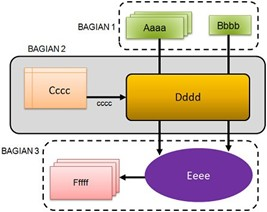
\includegraphics[width=0.8\textwidth]{gambar_desain_sistem.jpeg}
  \caption{Desain sistem dari solusi yang ditawarkan}
  \label{fig:desain_sistem}
\end{figure}

\begin{figure}[H]
  \centering
  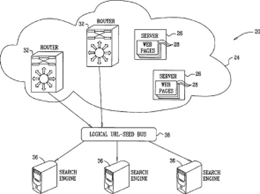
\includegraphics[width=0.8\textwidth]{gambar_kutipan.png}

  {\fontsize{12}{15}\selectfont\itshape Sumber: http://alamat-sumber.com/gambar.jpg\par}

  \caption{Contoh gambar kutipan}
  \label{fig:gambar_kutipan}
\end{figure}

\subsection{Bagian 1}

Disini penulis dapat menjelaskan lebih terperinci apa saja yang ada pada bagian ini. Apabila pembahasan memerlukan persamaan matematis, penulis dapat menuliskannya seperti pada Persamaan~(\ref{eq:binomial}).

\begin{equation}
  (x+a)^n = \sum_{k=0}^{n} \binom{n}{k} x^k a^{n-k}
  \label{eq:binomial}
\end{equation}

Persamaan~(\ref{eq:binomial}) menunjukkan teorema binomial yang merupakan dasar dari metode yang digunakan.

% --- Contoh tabel ---
Tabel~\ref{tab:contoh1} menunjukkan contoh penulisan tabel.

\begin{table}[H]
  \centering
  \begin{tblr}{colspec={c c c}}
    Kolom 1 & Kolom 2 & Kolom 3 \\
    Data 1-1 & Data 1-2 & Data 1-3 \\
    Data 2-1 & Data 2-2 & Data 2-3 \\
  \end{tblr}

  \vspace{4pt}
  {\fontsize{12}{15}\selectfont Sumber: Badan Pusat Pengolahan Data, 2026 \cite{buku_contoh}\par}

  \caption{Contoh penulisan tabel otomatis}
  \label{tab:contoh1}
\end{table}

\begin{equation}
  F = m \cdot a
  \label{eq:newton}
\end{equation}

\subsection{Bagian 2}

Disini penulis dapat menjelaskan lebih terperinci apa saja yang ada pada Bagian 2 ini.

\begin{table}[H]
  \centering
  \caption{Contoh penulisan tabel 2}
  \label{tab:contoh2}
  \begin{tabular}{|c|c|c|c|}
    \hline
    \rowcolor{gray!20}
    \textbf{Kolom 1} & \textbf{Kolom 2} & \textbf{Kolom 3} & \textbf{Kolom 4} \\
    \hline
    Data 1-1 & Data 1-2 & Data 1-3 & Data 1-4 \\
    \hline
    Data 2-1 & Data 2-2 & Data 2-3 & Data 2-4 \\
    \hline
  \end{tabular}
\end{table}

\subsection{Bagian 3}

Disini penulis dapat menjelaskan lebih terperinci apa saja yang ada pada Bagian 3 ini.

\begin{equation}
  \lim_{x \to c} f(x) = L
  \label{eq:limit}
\end{equation}

%============================================================
% BAB 4 - EKSPERIMEN DAN ANALISIS
%============================================================
\chapter{EKSPERIMEN DAN ANALISIS}

Uraian pada bab ini meliputi parameter eksperimen, karakteristik data, skenario ujicoba, tempat dan waktu eksperimen, spesifikasi peralatan ujicoba, cara penafsiran dan penyimpulan hasil proyek akhir.

\section{PARAMETER EKSPERIMEN}

Dalam eksperimen ini menggunakan persamaan sebagai berikut:

\begin{equation}
  y = mx + c
  \label{eq:linear}
\end{equation}
\begin{equation}
  \frac{y - y_1}{x - x_1} = \frac{y_2 - y_1}{x_2 - x_1}
  \label{eq:gradien}
\end{equation}
\begin{equation}
  v = v_0 + at
  \label{eq:glbb1}
\end{equation}
\begin{equation}
  s = v_0 t + \frac{1}{2}at^2
  \label{eq:glbb2}
\end{equation}
\begin{equation}
  v^2 = v_0^2 + 2as
  \label{eq:glbb3}
\end{equation}

\section{KARAKTERISTIK DATA}

Disini penulis dapat membahas karakteristik data lebih terperinci. Akan lebih baik jika penulis dapat memberikan alasan terhadap penggunaan data yang mempunyai karakteristik seperti itu.

\section{TEMPAT UJICOBA}

Disini penulis dapat membahas tempat pelaksanaan ujicoba lebih terperinci.

\section{WAKTU UJICOBA}

Disini penulis dapat membahas waktu pelaksanaan ujicoba pada penelitian lebih detail.

\section{SPESIFIKASI PERALATAN UJICOBA}

Disini penulis dapat membahas spesifikasi peralatan lebih terperinci. Peralatan dapat berupa perangkat keras, perangkat lunak, piranti elektronik, gadget, dan lain-lain.

\section{HASIL EKSPERIMEN}

\begin{table}[H]
  \centering
  \caption{Contoh tabel hasil eksperimen 1}
  \label{tab:hasil1}
  \begin{tabular}{|c|c|c|c|}
    \hline
    \rowcolor{gray!20}
    \textbf{Kolom 1} & \textbf{Kolom 2} & \textbf{Kolom 3} & \textbf{Kolom 4} \\
    \hline
    & & & \\
    \hline
    & & & \\
    \hline
  \end{tabular}
\end{table}

\begin{table}[H]
  \centering
  \caption{Contoh tabel hasil eksperimen 2}
  \label{tab:hasil2}
  \begin{tabular}{|c|c|c|c|}
    \hline
    \rowcolor{gray!20}
    \textbf{Kolom 1} & \textbf{Kolom 2} & \textbf{Kolom 3} & \textbf{Kolom 4} \\
    \hline
    & & & \\
    \hline
    & & & \\
    \hline
  \end{tabular}
\end{table}

\begin{table}[H]
  \centering
  \caption{Contoh tabel hasil eksperimen 3 dengan parameter eksperimen yang cukup banyak sehingga nama tabel panjang}
  \label{tab:hasil3}
  \begin{tabular}{|c|c|c|c|}
    \hline
    \rowcolor{gray!20}
    \textbf{Kolom 1} & \textbf{Kolom 2} & \textbf{Kolom 3} & \textbf{Kolom 4} \\
    \hline
    & & & \\
    \hline
    & & & \\
    \hline
  \end{tabular}
\end{table}

\section{ANALISIS HASIL EKSPERIMEN}

Disini penulis dapat membahas analisis hasil eksperimen lebih terperinci. Analisis hasil eksperimen seharusnya menjawab hipotesa bahwa solusi yang diajukan pada Tujuan dapat menyelesaikan permasalahan.

\begin{figure}[H]
  \centering
  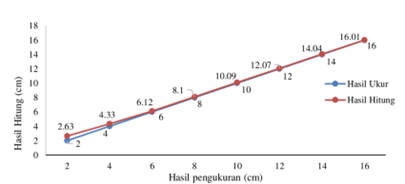
\includegraphics[width=0.75\textwidth]{gambar_hasil1.png}
  \caption{Contoh gambar hasil eksperimen 1}
  \label{fig:hasil1}
\end{figure}

Grafik pada Gambar~\ref{fig:hasil1} menunjukkan hubungan antara pengukuran dan perhitungan dari Persamaan~(\ref{eq:linear}).

\begin{figure}[H]
  \centering
  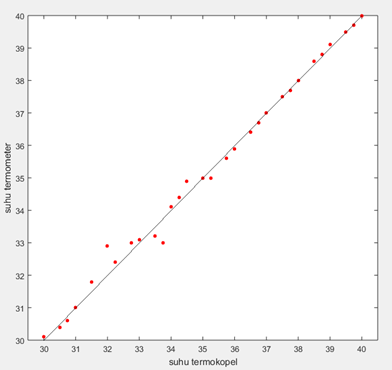
\includegraphics[width=0.75\textwidth]{gambar_hasil2.png}
  \caption{Contoh gambar hasil eksperimen 2 dengan nama gambar yang cukup panjang sehingga diperlukan penataan yang baik dalam daftar gambar}
  \label{fig:hasil2}
\end{figure}

Grafik pada Gambar~\ref{fig:hasil2} menunjukkan hubungan antara sensor suhu 1 dan sensor suhu 2 yang dibentuk dari Persamaan~(\ref{eq:gradien}).

%============================================================
% BAB 5 - PENUTUP
%============================================================
\chapter{PENUTUP}

Bab 5 memuat penjelasan ringkas dari apa yang telah ditulis dari Bab 1 sampai Bab 4.

\section{KESIMPULAN}

Berikan kesimpulan terhadap: (1) \textit{Problem} dan tingkat urgensi, (2) solusi yang penulis tawarkan, (3) orisinalitas pada proyek akhir ini, (4) desain sistem, serta (5) eksperimen dan kinerja sistem terhadap permasalahan.

\section{SARAN}

Berikan saran terhadap keterbatasan solusi untuk pengembangan dan peningkatan solusi dalam menjawab permasalahan di masa mendatang.

%============================================================
% DAFTAR PUSTAKA
%============================================================
\cleardoublepage
\addcontentsline{toc}{chapter}{DAFTAR PUSTAKA}

\bibliographystyle{IEEEtran}
\bibliography{references}

%============================================================
% LAMPIRAN
%============================================================
\cleardoublepage
\appendix
\addcontentsline{toc}{chapter}{LAMPIRAN}

\chapter*{LAMPIRAN}
\renewcommand{\thesection}{\Alph{section}}

Lampiran berisi informasi yang menunjang bahasan dalam Buku Proyek Akhir, seperti data yang cukup banyak, \textit{datasheet}, pembuktian matematis, dan lain-lain.

\end{document}